\section{Soudní znalectví}
\subsection{Soudní znalectví a soudní inženýrství}
Soudní znalectví je teoreticko-aplikační obor lidské činnosti, v rámci kterého se realizuje znalecká činnost.

Soudní inženýrství původně bylo vytvořeno jako odborně-vědecká znalostní, teoretická a metodologická nadstavba k soudnímu znalectví. Dnes je soudní inženýrství
vědecká disciplína, která se zabývá znaleckým a expertním posuzováním různorodých typů objektů v inženýrských oborech, je typem znalostního a systémového
inženýrství, kde se uplatňují znalosti z různých vědních oborů.

Rozdíl mezi těmito dvěma pojmy je tedy v tom, že soudní znalectví je teoreticko-aplikační obor, v rámci kterého se praktikuje znalecká činnost téměř ve všech
oblastech činnosti. Soudní inženýrství je pak datová, informační, metodologická nadstavba znalectví v klasických inženýrských oborech.

\subsection{Soustava znalectví}
\begin{figure}[h]
    \centering
    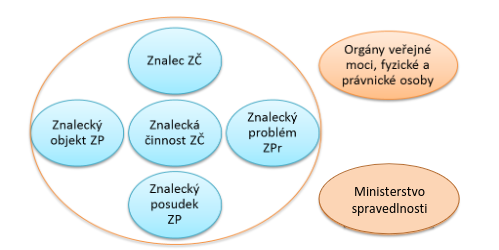
\includegraphics[width=0.8\textwidth]{images/soustava.png}
    \caption{Soustava znalectví}
    \label{fig:soustava_znalectvi}
\end{figure}
\subsubsection*{Znalec}
Pod tímto pojmem rozumíme všechny právnické nebo fyzické osoby, které mohou vykonávat znaleckou činnost. Každý znalec na základě zadání a analýzy situace 
formuluje znaleckém objektu znalecký problém, realizuje jeho řešení a zpracuje znalecký posudek.
\subsubsection*{Znalecký objekt}
Objekt, jenž je předmětem konkrétního zájmu určitého subjektu požadujícího o objektu vypracování znaleckého posudku.
\subsubsection*{Znalecký problém - ZPr}
Odborný problém, který souvisí s typem a stavem zanleckého objektu, se stavem jeho okolí a zájmem o objekt, daný zájmem subjektu pro který se posudek 
vypracovává.
\subsubsection*{Znalecká činnost}
Proces získávání, zpracování a předávání informací, s cílem vyřešit ZPr a zpracovat znalecký posudek.
\subsubsection*{Znalecký posudek}
Výsledek znalecké činnosti, který obsahuje:
\begin{itemize}
    \item Otázky týkající se objektu
    \item Znalecký problém
    \item Nálezy o posuzovaném objektu
    \item Metody řešení
    \item Řešení znaleckého problému
    \item Výsledky
    \item Shrnutí výsledků do odpovědí na otázky
\end{itemize}

\subsubsection*{Podstatné prvky okolí}
Orgány veřejné moci, fyzické a právnické osoby zadávají znalcům znalecké úkoly a zpětně využívají výsledky jejich činnosti, ať už pro potřeby rozhodování
v řízení před orgány veřejné moci nebo provádění právních úkonů.

Ministerstvo spravedlnosti v čele s ministrem organizuje a řídí znaleckou činnost, rozhoduje o vzniku a zániku oprávnění pro ZČ, vede seznam znalců,
dohlíží na výkon ZČ.

\section{Pojmy cena  hodnota z pohledu teorie oceňování}
\subsection{Pojmy cena a hodnota podle mezinárodních zvyklostí}
Dle mezinárodních zvyklostí se pojem cena používá výhradně pro označení nabízené nebo skutečně zaplacené částky peněz za určitý statek nebo službu.
Standardně se jedné o historickou cenu, která na trhu existovala či existuje. Pojem lze vztahovat i k prognózovanému vývoji trhu, nebo ke kalkulacím, 
které si subjekty tvoří samy pro budoucí období.

Hodnota je při oceňování peněžitá částka, která bere v ohled vymezený zájem o objekt. Je objektu přiřazena na základě kvantifikace užitku, stanoveného z 
pohledu konkrétního subjektu(stát, věřitel, kupující se zvláštním zájmem) nebo skupiny subjektů(vlastníka a potenciálních vlastníků...). Obecně ji jde vymezit
takto: Hodnota je peněžitá částka, která z hlediska vymezeného zájmu o objektu vyjadřuje kvantifikovaná projev objektu ve prospěch určitého subjektu nebo skupiny subjektů.

\subsection{Typy cen}
\subsubsection*{Podle stavu transakce}
Lze je rozlišovat na ceny nabízené, poptávané a sjednané. Nabízené stanovuje prodávající, poptávané kupující a sjednaná cena je taková kdy došlo ke 
shodě mezi prodávajícím a kupujícím.
\subsubsection*{Podle časovéh okamžiku}
Rozlišujeme ceny historické, současné a prognózované. Historické ceny jsou ceny, které byly nabízeny, poptávány nebo zaplaceny v minulosti, 
současné ceny jsou ceny nabízené, poptávané či placené v současnosti a prognózované jsou ceny stanovené na základě historického vývoje cen nebo kalkulací
výrobce pro budoucí období.
\subsubsection*{Podle způsobu zveřejnění}
Dělíme je na zveřejněné a tajné
\subsubsection*{Podle volnosti}
Ceny mohou být volné a regulované. U volných tak není státem stanoveno omezení pro sjednání výše ceny. U regulovaných tak je státem regulován způsob stanovení
ceny. 
\subsubsection*{Podle specifických podmínek}
Při sjednávání lze stanovit cenu dražební, cenu zvláštní obliby(zohledňuje zvláštní vztah prodávajícího nebo kupujícího k danému majetku), cenu uzavřenou
v tísni(cena zohleňující mimořádné okolnosti v době jejího uzavření)

\subsection{Typy hodnot}
\subsubsection*{Podle metody zjištění}
Nákladová(náklady na pořízení majetku a jeho opotřebení), výnosová(zohledňuje dosažitelné výnosy z majetku), porovnávací(zohledňuje dosahovné ceny blízkých
substitutů daného typu majetku)
\subsubsection*{Podle subjektu}
Z pohledu vlastníka, z pohledu kupujícího se zvláštním zájmem(hodnota sloučení), investora(investiční hodnota), zástavního věřitele(zástavní hodnota), státu(administrativní hodnota)
\subsubsection*{Podle vstupních údajů}
Hodnota založená na analýze trhu(tržní hodnota) a hodnota nezaložená na analýze trhu(investiční či administrativní hodnota)

\section{Hodnota hmotných věcí}
Nemám nejmenší tušení kde tohle vzít, nikde to není v těch jeho plesnivých skriptech
\subsection{Charakterisky věci}
Funkčnost, životnost, kvalita zpracování, bezpečnost
\subsection{Prvky okolí}
Provedení a stav objektu, užitečnost objektu ve vztahu k jeho cílovému chování a užitek subjektu z jehož pohledu se ocenění provádí

\begin{figure}[h]
    \centering
    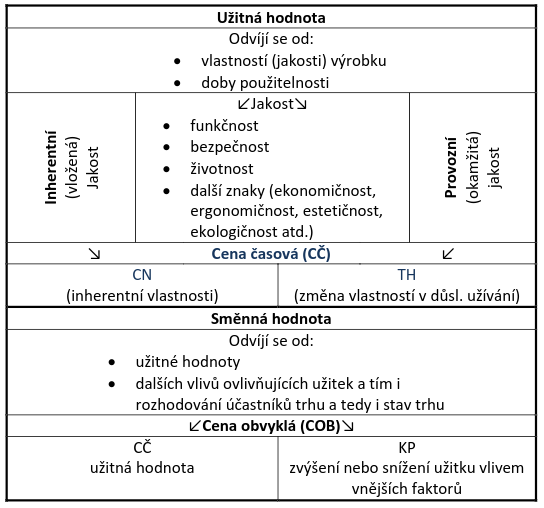
\includegraphics[scale = 0.5]{images/hodnota.png}
    \caption{Užitná hodnota}
    \label{fig:hodnota_hmotnych_veci}
\end{figure}

\section{Nákladový přístup ke stanovení hodnoty majetku}
Hodnota nákladová, též věcná či časová, je hodnota založená na posouzení výchozí a provozní jakosti výrobku.\\
\begin{equation}
    HČ = HN\cdot ZU
\end{equation}\\
Kde HN je výchozí hodnota, což je hodnota reflektující náklady na pořízení objektu, bere se jako cena, za kterou bylo možné objekt pořídit jako nový
k datu ocenění. ZU je zbytková užitnost, reflektující zbytek užitečného života věci. 
\begin{equation}
    ZU = \frac{100\%\cdot (100-ZA)\cdot (100 \pm PS)}{10^6}
\end{equation}
\subsection{Určování výchozí hodnoty}
Pro sériově vyráběné věci se vychází z aktuální ceny nového produktu, pokud tento produkt již není v prodeji, může se vzít cena podobného produktu od 
stejného výrobce, přičemž se vezme v potaz technický rozdíl pomocí koeficientu technické úrovně.
Pokud považujeme stavby za věci vyráběné na zakázku tak můžeme uplatnit tyto metody určení výchozí hodnoty:
\begin{itemize}
    \item Individuální cenová kalkulace - zjištění materiálových nákladů, nákladů na mzdy, pořizovacích nákladů, nákladů vynaložených zhotovitelem atd.
    \item Podrobný položkový rozpočet -  Pro jednotlivé položky rozpočtu je stanoven kalkulační vzorec, spotřeba materiálu na jednotku konstrukce, časová náročnost prací
    \item Výpočet pomocí agregovaných položek - Principem této metody je, že hodnota konstrukcí stavby se zjistí pomocí tzv. agregovaných položek, kdy v jedné položce rozpočtu jsou již sloučeny náklady na veškeré
    související stavební práce, viz příklad níže, kde v 1 položce je agregováno 15 složek stavebních prací.
    \item Propočet ceny pomocí cenových ukazatelů - Výchozí hodnota se stanoví na základě porovnání oceňované stavby s obdobnou stavbou, jejíž pořizovací náklady známe.
\end{itemize}

\subsection{Amortizační stupnice}
\subsubsection*{Stavby}
\begin{itemize}
    \item Lineární - Opotřebení stavby jako celku. Každý rok se opotřebení zvyšuje o stejnou hodnotu. Při životnosti 100 let je to 1\% ročně.
    \item Semikvadratická - nic o ní nepíše
    \item Kvadratická - nic o ní nepíše
    \item Kusínova - nic o ní nepíše
\end{itemize}
\subsubsection*{Stroje}
\begin{itemize}
    \item Lineární se zbytkem - Hodnota se snižuje a na konci je nějaká zbytková, moc tam o tom není
    \item Nelineární - nic o nich nepíše
\end{itemize}

\subsection{Délka užitečného života}
Dynamická veličina vyjadřující dobu, po kterou ještě lze očekávat nedosažení mezního stavu.

\subsection{Mezní stavy}
\subsubsection*{Mezní stav technický}
Příčiny mezního stavu i důvody pro ukončení životnosti mají technický charakter. Například vznikne neopravitelná porucha
\subsubsection*{Mezní stav technicko-ekonomický}
Příčina mezního stavu má technický charakter, ale důvod pro ukončení životnsoti má ekonomický charakter. Například nastala porucha, která je opravitelná,
ale oprava je ekonomicky nevýhodná(oprava je dražší jak nová koupě).
\subsubsection*{Mezní stav ekonomický}
Příčina mezního stavu i důvody pro ukončení životnosti mají ekonomický charakter. Nastane kdy užitek poklesne pod přijatelnou úroveň. Například stará technologie
se už nevyplatí kvůli nutnosti ji často opravovat.

\section{Výnosový přístup ke stanovení hodnoty majetku}
\subsection{Pojmy}
\begin{itemize}
    \item Úrok U[Kč]- částka, která přibude k jistině J za dobu t při úrokové míře u
    \item Úroková míra u[\%]- určuje kolik \% z jistiny J činí úrok za určité období, obvykle rok.
    \item Úroková sazba i[-] - setinné vyjádření úrokové míry \( i = \frac{u}{100}\)
    \item Úročitel q[-] - udává, na kolik vzroste úrokem 1 koruna za rok při dané úrokové sazbě \( q = 1 + i\)
    \item Diskontní míra r[\%] - je procentní sazba, kterou se diskontují (přepočítávají) budoucí čisté výnosy z nemovité věci (zisky) v jednotlivých obdobích na
    současnou hodnotu. Používá se při výnosovém oceňování
    \item Míra kapitalizace p[\%] - je procentní sazba stanovená v příloze oceňovací vyhlášky. Používá se při oceňování výnosovým způsobem podle oceňovací
    vyhlášky. 
\end{itemize}
\subsection{Výnosová hodnota}
Je dána velikostí kapitálu, jenž by při uložení na danou úrokovou míru v budoucnu umožňoval vyplatit takové částky, které by byly rovny výnosům, které
by přinášela nemovitost. Nejčastěji využíván výpočet pro věčnou rentu
\subsection{Základní úvahy}
Při výnosovém oceňování se na nemovitou věc nahlíží jako na investici, která může přinášet výnos v podobě nájemného, a tedy i zisk. Hodnota věci se
zjistí jako součet budoucích příjmů. Jelikož tyto příjmy budou vznikat v budoucnosti, jejich současná hodnota se zjistí tzv. kapitalizací.

\subsection{Výpočet výnosové hodnoty}
\begin{equation}
    PV = \sum_{t=1}^{n}\frac{FV_t}{q^t}
\end{equation}
Kde FV je budoucí hodnota, PV je současná hodnota, q je úročitel a t je doba, na kterou se kapitál ukládá.
\subsection{Věčná renta}
\begin{equation}
    PV = \frac{FV}{i}
\end{equation}
Věčná renta se dá použít pokud se dá očekávat že budoucí výnosy budou nevýznamně proměnné.

\section{Porovnávací přístup ke stanovení hodnoty majetku}
Při aplikaci porovnávacího způsobu ocenění se hodnota oceňovaného objektu dovozuje z hodnoty srovnatelných objektů, pro
které jsou známé jejich dosažené prodejní ceny. Vycházíme tedy z hodnoty, kterou konkrétní prodávající a kupující přiřadili porovnatelným objektům při směně (při
jejich prodeji a koupi) formou sjednané ceny.
\subsection{Omezení metody}
Lze ji použít pouze když:
\begin{enumerate}
    \item existuje dostatečně velký soubor porovnatelných věcí, pro které ceny
    známe. Z jednotlivé ceny by totiž nebylo možno usuzovat na směnnou
    hodnotu oceňované věci, protože do výše ceny věci porovnatelné se mohly
    promítnout i mimořádné vlivy, které z jednoho pozorování trhu nelze zjistit,
    \item rozdíly užitných vlastností věci oceňované a porovnatelných nejsou příliš
    významné, protože jinak by je bylo velmi obtížné (ne-li nemožné)
    kvantifikovat
\end{enumerate}
\subsection{Metoda přímého porovnání}
\begin{enumerate}
    \item Vyhledají se nemovitosti, které jsou porovnatelné s nemovitostí
    oceňovanou a pro které jsou známé i dosažené prodejní, příp. alespoň
    nabídkové ceny. Přiměřeně se zjistí jejich vlastnosti a údaje se zpracují do
    databáze.
    \item Stanoví se kritéria pro porovnávání, přičemž etalonem pro porovnávání jsou
    vlastnosti oceňovaného objektu a jeho okolí.
    \item Každá nemovitá věc z databáze se porovná s nemovitou věcí oceňovanou a
    rozdíl užitných hodnot se vyjádří koeficientem odlišnosti, kterým se upraví
    známé prodejní ceny nemovitých věcí v databázi porovnatelných objektů.
    \item Dosažitelná cena oceňovaného objektu (hodnota porovnávací HPOR) se
    dovodí ze zpracování souboru upravených cen porovnatelných objektů.
\end{enumerate}
\begin{figure}[h]
    \centering
    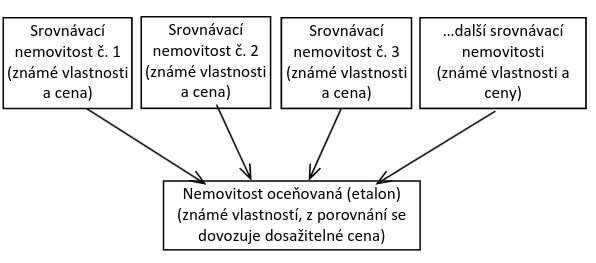
\includegraphics[scale=0.5]{images/porovnani.png}
    \caption{Metoda přímého porovnání}
    \label{fig:porovnani}
\end{figure}
\subsection{Metoda nepřímého porovnání}
\begin{enumerate}
    \item Stejně jako výše se porovnatelné nemovitosti, pro které jsou známé jejich
    prodejní ceny. Přiměřeně se zjistí jejich vlastnosti a údaje se zpracují do
    databáze.
    \item Vymezí se vlastnosti etalonového objektu a stanoví se kritéria pro
    porovnávání.
    \item Z porovnání vlastností srovnávacích objektů oproti etalonu se dovodí cena
    standardního objektu obdobně jako u přímého porovnání.
    \item Dosažitelná cena oceňovaného objektu (hodnota porovnávací HPOR) se
    dovodí z ceny dovozené pro etalon a z porovnání vlastností oceňovaného
    objektu a etalonu.
\end{enumerate}
\begin{figure}[h]
    \centering
    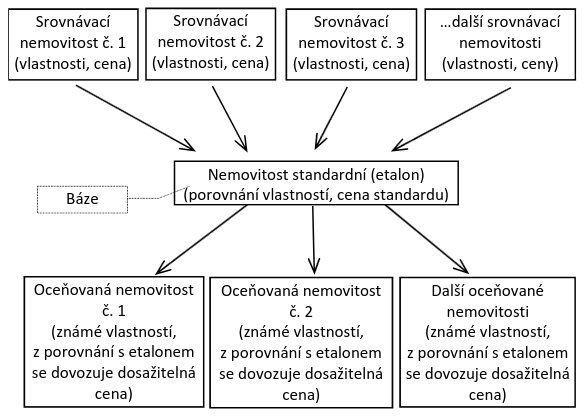
\includegraphics[scale=0.5]{images/porovnani2.png}
    \caption{Metoda nepřímého porovnání}
    \label{fig:porovnani2}
\end{figure}
\subsection{Prodej podle koeficientu prodejnosti}
Vezmeme objekt, jehož cenu chceme stanovit, najdeme podobné objekty, které jsou srovnatelné. Ideálně stejné, pokud však ne tak se použije koeficient
technické úrovně, u všech se spočítá hodnota časová a cena za kterou se projekty prodávají. Koeficient prodejnosti se zjistí jako průměr podílů ceny, za kterou
jsou objekty prodávány a jejich časové hodnoty. Tento koeficient se pak použije k výpočtu ceny oceňovaného objektu. Tržní hodnota se pak určí jako 
součin hodnoty časové a koeficientu prodejnosti.

\section{Způsob stanovení výše škody}
Majetková újma představuje jakoukoliv ztrátu na majetku. Ta se dělí na škodu skutečnou a ušlý zisk. Odčiňuje se restitucí tvz. obnovením původního stavu
majetku. U věci se primárně požaduje její uvedení do původního stavu (restituce naturální) nebo nahrazení újmy penězi (restituce relutární)\\
Nemajetková újma představuje újmu způsobenou protiprávním zásahem do osobních práv člověka (příp. obdobných práv právnické osoby). Typicky se jedná
o zásah do zdraví, cti, soukromí osoby. Náhrada za nemajetkovou újmu se poskytuje formou zadostiučiněním (satisfakcí). Lze-li újmu skutečně
a dostatečně odčinit jinak než penězi, použije se takový způsob, v opačném případě se odčiní peněžitou náhradou. \\
Skutečná škoda představuje újmu, která vznikla tím, že se hodnota majetku poškozeného snížila.\\
Ušlý zisk představuje újmu, která vznikla tím, že se hodnota majetku poškozeného nezvýšila, ačkoliv měla.\\
\subsection{Právní úprava náhrady škody}
K tíži poškozeného nesmí jít:
\begin{itemize}
    \item znehodnocení věci její opravou (oproti původnímu stavu), tedy skutečnost,
    že by poškozený měl po opravě věc nižší ceny než před vznikem škody,
    \item okolnosti, jež jsou nahodilé a bez souvislosti s příčinou vzniku škody (např.
    nezaplacení prací, jež si poškozený provádí sám)
\end{itemize}
K tíži škůdce nesmí jít:
\begin{itemize}
    \item zhodnocení věci její opravou (oproti původnímu stavu), rozumí se takové,
    které má skutečný vliv na cenu věci
    \item nehospodárnost provedené opravy, tedy skutečnost, že na opravu byly
    vynaloženy neúměrně vysoké nebo neúčelné náklady.
\end{itemize}
Zohlednitelná cena zbytků by měla být vždy stanovena objektivně, tak aby mohla být naplněna podmínka uvedení do původního stavu.
\subsection{Stanovení přímé škody}
Provedení opravy není ekonomické pokud jsou náklady na opravu(NO) větší jak cena věci před poškozením(C1). Pak se musí zajistit aby si poškozený mohl
pořídit věc stejné kvality a hodnoty. Ve výši náhrady je nutno zohlednit cenu zbytků, protože tato hodnota poškozenému zůstane.\\
Pokud provedení opravy ekonomické není použije se vztah:
\begin{equation}
    VÚ = C1 - CZ
\end{equation}
Kde VÚ je výše újmy, C1 je cena věci před poškozením a CZ je cena zbytků.\\

Pokud však je provedení opravy ekonomické, tedy \(NO < C1\), pak se musí zajistit aby poškozený po opravě měl věc stejné kvality a hodnoty. Pak je nutno
stanovit NO(posoudit zda byla oprava provedena účelně), zda se provedením opravy nezmění obbyklá cena věci, tedy zda se cena věci po opravě(C2) není větší
nebo menší než C1 a musí se zohlednit cena zbytků.\\
Pak je použit vztah:\\
\begin{equation}
    VÚ = NO + (C1 - C2) - CZ
\end{equation}

\section{Právní úprava znalecké činnosti}
Vykonávat znaleckou činnost může znalec, znalecké kanceláře či znalecké ústavy. Znalec ji může vykonávat samostatně nebo jako zaměstnanec či společník
znalecké kanceláře.
Vykonávat znaleckou činnost může znalec vykonávat pokud:
\begin{itemize}
    \item Je odborně způsobilý k výkonu znalecké činnosti v daném oboru a odvětví
    \item Je bezúhonný
    \item Má odpovídající materiálně technické zázemí a přístrojové vybavení
    \item Je svéprávný
    \item Nebyl v posledních 3 letech před podáním zádosti o zápis potrestán pokutou nejméně 100 000Kč
    \item Není na základě pravomocného rozhodnutí soudu v úpadku
    \item Má kontaktní adresu na území ČR 
    \item Po splnění předchozích podmínek složil slib do rukou ministra spravedlnosti
\end{itemize}

\subsection{Zásady výkonu znalecké činnosti}
Musí se řídit slibem znalce, kde se zavazuje k tomu, že bude při ZČ dodržovat právní předpisy, bude ZČ vykonávat dle svého nejlepšího vědomí a svědomí,
nezávisle a nestranně, bude využívat svách znalostí a dbát o jejich rozvoj a zachová mlčenlivost o skutečnostech o nichž se při výkonu ZČ dozvěděl.
\subsubsection*{Povinnosti znalce}
Bude vykonávat ZČ pouze ve svém oboru, s odbornou péčí, nezávisle, nestranně, ve sjednané nebo stanovené době, osobně.
\subsection{Oprávnění provést úkon}
Nelze pochybovat o jeho nepodjatosti. Nesmí odmítnout pokud mu OVM zadá vykonat znalecký úkon, odmítnout může pouze pokud má pozastaveno oprávnění,
nedovolují mu to zdravotní okolnosti či závažná rodinná situace, nebo tak stanoví jiný zákon.
\section{Znalecký posudek}
ZP se podává v listinné, elektronické nebo ústní podobě. Podaný ZP musí být pravdivý, úplný a přezkoumatelný.\\
Struktura ZP musí obsahovat:
\begin{itemize}
    \item Titulní stanu
    \item Zadání
    \item Výčet podkladů
    \item Nález
    \item Posudek
    \item Odůvodnění v rozsahu umožňujícím přezkoumatelnost
    \item Závěr
    \item Přílohy potřebné k zajištění přezkoumatelnosti
    \item Znaleckou doložku
    \item Otisk znalecké pečeti
\end{itemize}
\subsection{Titulní strana}
Musí obsahovat:
\begin{itemize}
    \item Označení znalce a zadavatele
    \item Číslo jednací zadavatele, pokud je zadavatelem OVM a pokud číslo sdělil
    \item Označení "znalecký posudek" a číslo položky, pod kterou je ZP zapsán v evidenci posudků
    \item Stručný popis předmětu ZP
    \item Obor a odvětví, případně specializaci
    \item Číslo vyhotovení a celkový počet vyhotovení
    \item Datum zpracování ZP
\end{itemize}
\subsection{Zadání}
Musí obsahovat:
\begin{itemize}
    \item Odbornou otázku zadanou zadavatelem
    \item Údaj pro jaké účely má být ZP použit
    \item Skutečnosti sdělené zadavatelem
\end{itemize}
\subsection{Výčet podkladů}
Musí obsahovat:
\begin{itemize}
    \item Popis postupu znalec při výběru zdrojů dat
    \item Výčet vybraných zdrojů a jejich popis
\end{itemize}
\subsection{Nález}
Musí obsahovat:
\begin{itemize}
    \item Popis postupu znalce při sběru nebo tvorbě dat a při jejich zpracování
    \item Výčet těchto dat
\end{itemize}
\subsection{Posudek}
Musí obsahovat:
\begin{itemize}
    \item Popis postupu znalce při analýze dat
    \item Výsledky analýzy dat
\end{itemize}
\subsection{Odůvodnění}
Musí obsahovat:
\begin{itemize}
    \item Interpretaci výsledků analýzy dat
    \item Kontrolu postupu znalce
\end{itemize}
\subsection{Závěr}
Musí obsahovat:
\begin{itemize}
    \item jednoznačné odpovědi na položené otázky
    \item případně skutečnosti snižující přesnost závěru
\end{itemize}
\subsection{Poslední strana posudku}
Musí obsahovat:
\begin{itemize}
    \item Zda byl k zpracování přizván konzultant
    \item za byla sjednána smluvní odměna
    \item znaleckou doložku
    \item případně též doložku znalce o tom, že si je vědom následků vědomě
    nepravdivého znaleckého posudku, kterou umístí před znaleckou doložku,
    \item otisk znalecké pečeti
    \item datum a podpis osob
\end{itemize}
\section{Praktický výkon znalecké činnosti}
\includegraphics*[scale = 0.75]{images/vykon.png}
\section{Podíl znalce na zajištění důkazů}
Dokazování je myšlenková forma, spočívající v tom, že pomocí logického postupu dovozujeme, že určitá zjišťovaná skutečnost(důkaz) vyplývá 
z určitých argumentů(důkazních prostředků).
Důkazní prostředek je způsob jímž lze zjistit stav věci, např. výslech svědků, znalecký posudek, vyjádření orgánů, fyzických a právnických osob atd.
Důkazem je pak výsledek dokazování, konkrétní poznatek, který orgán provádějící dokazování získal o předmětu důkazu z důkazního procesu procesním dokazováním.
\subsection{Zvláštní způsoby dokazování}
\begin{itemize}
    \item konfrontace - slouží k odstranění rozporů ve výpovědích
    \item rekognice - slouží k identifikaci osoby nebo věci
    \item vyšetřovací pokus - slouží k prověření nebo upřesnění zjištěné skutečnosti nebo k zjištění nové skutečnosti
    \item rekonstrukce - obnovení původního stavu objektů a jejich okolí
    \item prověrka na místě - slouží k doplnění nebo upřesnění údajů, které se vztahují k určitému místu
\end{itemize}
\subsection{Obyklé důkazní prostředky}
\begin{itemize}
    \item Výpovědi obviněného a svědků
    \item Věci a listiny důležité pro trestní řízení
    \item Znalecký posudek
    \item Ohledání
\end{itemize}
\subsection{Podíl znalce na dokazování}
Podílí se buď na zajištění jiného typu důkazu nebo zpracováním znaleckého posudku. V prvním případě je znalec přítomen především proto, aby svými odbornými
znalostmi přispěl k zjištění všech okolností, zejména těch, které budou potřebné pro eventuální další znalecké zkoumání. 